\chapter{Trabalhos Correlatos}\label{sec:relacionados}
Os trabalhos relacionados são discutidos neste capítulo e está organizado da seguinte forma.  Na Seção \ref{sec:edc} analisa as principais extrações de características encontradas na literatura para o processamento da expressão facial. Na Seção \ref{sec:arct} avalia os trabalhos correlatos categorizados pelas arquiteturas de RNC. Na Seção \ref{sec:apl} é comentado as aplicações para o reconhecimento de emoção por expressão facial e enquanto a Seção \ref{sec:cons} faz um resumo a respeito deste capítulo.


\section{Preparação dos dados}\label{sec:dataprepared}
Os problemas de classificação em geral, seja de imagem, vídeo, áudio ou qualquer tipo, tradicionalmente sofrem pela ausência de dados. Algoritmos de aprendizagem de máquina requerem quantidade de dados expressivos para apresentar soluções com desempenho satisfatório, especificamente as redes neurais profundas. Raramente há dados disponíveis e que sejam suficientes para treinar e validar uma rede neural de convolução, vale ressaltar que cada problema tem sua particularidade, isto é, quanto maior a complexidade mais dados são necessários. 

Contudo, a comunidade de reconhecimento de emoção para amenizar esse problema utiliza a técnica de aumento de dados e multiplicação de imagens. Essa técnica consiste na geração de cópias de uma imagem original, que contém uma expressão facial, para gerar imagens duplicadas. Entretanto, tais imagens duplicadas são diferentes da imagem original, justamente por possuir alterações na posição da face com leves rotações da mesma, variação da intensidade das cores e redimensionamento com aplicação de \textit{zoom}. As imagens aumentadas são usadas durante o treinamento contribuindo para a rede neural aprender a reconhecer emoção em diferentes rotações, intensidade de iluminação e escala. 

Os trabalhos de \cite{art4, art6, art7, art8, art11} e \cite{art15} utilizaram a técnica de aumento de dados. A técnica foi configurada para aumentar entre 5 a 10 vezes cada imagem original. Sendo assim, a base de dados original foi ampliada em até 10 vezes, gerando um ganho considerável dos dados. Tais trabalhos alcançaram boas taxas de reconhecimento em que o \emph{fine tuning} dos modelos possuem generalização adequada e não apresentando \emph{overfitting} e \emph{underfitting}. O resultado expressivo foi viabilizado pela técnica de aumento de dados justamente pela rede ser treinada e validada com maiores quantidades de dados. 
%tais imagens duplicadas possuem alterações na posição da face aplicando leves rotações da imagem original gerando novas imagens válidas tanto para treinamento como para validação.      

%\section{Metodologia de Treinamento e Validação}\label{sec:trainingValidationMethodology}


\section{Extração de Característica}\label{sec:edc}
Uma etapa essencial durante o processo de classificação de imagem é a extração de característica. A extração de característica é sucintamente enfatizada na Seção \ref{sec:pci} e tem como finalidade destacar ou retirar as formas mais relevantes da imagem que são cruciais para a separação das classes. A seguir, os principais tipos de extração de características empregados para o reconhecimento de emoção por expressão facial são analisados.

\subsection{Extração Geométrica}
A extração de características geométrica consiste na obtenção de pontos faciais ilustradas pela Figura \ref{fig:geometrica}. As características geométricas tem como finalidade capturar as deformações na face causadas pela ativação dos músculos a partir dos pontos faciais \citep{art11}. Esses pontos faciais podem ser mapeados pelos seguintes métodos: \cite{yu2016face} e \cite{yu2014consensus}.
A extração geométrica é uma abordagem que realiza medições entre diversas partes da face tais como:

\begin{enumerate}[label=(\roman*)]
\item Altura da sobrancelha esquerda/direita (distância vertical entre o ponto mais superior da sobrancelha e centro do olho);  
\item Altura da pálpebra esquerda/direita (distância vertical entre o ponto mais superior do olho e parte inferior do olho);  
\item Altura do nariz (distância vertical entre o ponto mais inferior do olho para o nariz e centro de ambos os olhos);  
\item Largura do nariz (distância horizontal entre os pontos do nariz mais à esquerda e à direita);  
\item Altura do lábio superior (distância vertical entre o ponto mais superior e o centro da boca); 
\item Altura do lábio inferior (distância vertical entre o ponto mais inferior e o centro da boca); 
\item A distância do ponto da boca mais a esquerda para o centro da boca; 
\item E por fim, a distância do ponto da boca mais a direita para o centro da boca.
\end{enumerate}

A extração geométrica é amplamente empregada nas abordagens tradicionais de aprendizado de máquina, isto é, abordagens que não utilizam as redes neurais de convolução. Todavia, o trabalho de \cite{art11} realiza a extração geométrica concatenando com a RNC e obteve um pequeno ganho na taxa de precisão de 1\%. Um diagrama da sua abordagem é ilustrada na Figura \ref{fig:yun-customizing}. No entanto, a combinação entre a extração geométrica e RNC, obviamente, aumenta o custo computacional devido a outros algoritmos serem executados como o mapeamento dos pontos faciais e as suas distâncias. Caso o foco do reconhecedor de emoções for aplicações em cenários reais, provavelmente, não é viável a concatenação devido o aumento na taxa de reconhecimento ser baixo, portanto não compensada pelo aumento do custo computacional, pois tais cenários requerem classificação instantânea e em tempo real.

\begin{figure}
\centering
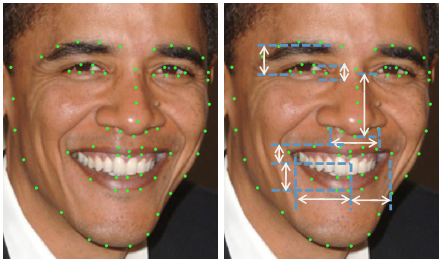
\includegraphics[scale=0.45]{figuras/tipogeo.png}
\caption{Extração dos pontos faciais para características geométrica}
\label{fig:geometrica}
\end{figure}

\begin{figure}
\centering
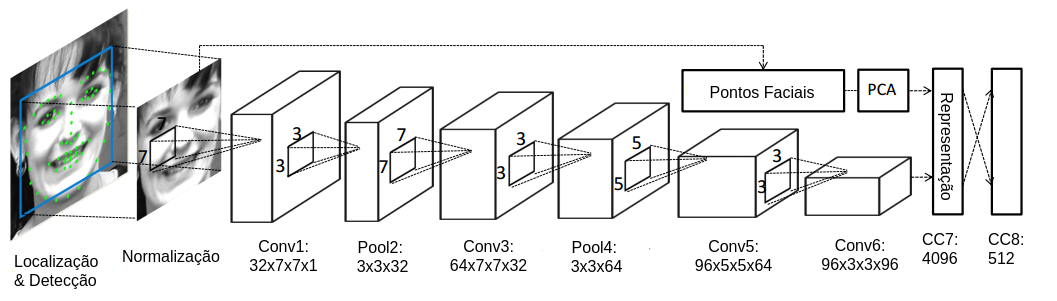
\includegraphics[scale=0.48]{figuras/yun-customizing.png}
\caption{Concatenação dos pontos faciais com uma rede neural de convolução}
\label{fig:yun-customizing}
\end{figure}



\subsection{Extração Aparente}
A extração de característica aparente considera as sub-regiões faciais, principalmente próximas da boca e dos olhos, como características essenciais para a classificação, diferentemente, das características geométricas que foca na captura das deformações dos pontos faciais e possui como desvantagem não considerar as mudanças aparentes causadas por essas deformações capturadas \citep{art11}. A  extração aparente foi amplamente estudada por \cite{ekman1994}, encontrando 96 unidades de ações (ou sub-regiões) na face correspondentes a movimentação de diversos músculos relacionada a uma determinada emoção. A RNC está habilitada naturalmente a realizar a extração de característica aparente, sendo assim, o processo de aprendizado está associado a descoberta de quais as sub-regiões da face mais relevantes para determinar qual a emoção está emitida em uma face. A Figura \ref{fig:aparente} ilustra as sub-regiões de uma face que são interessantes para a classificação depois de um processo de aprendizado.


\begin{figure}
\centering
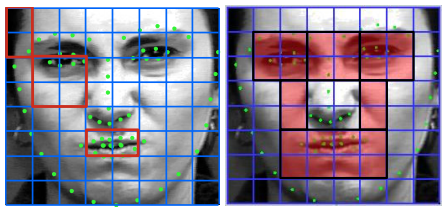
\includegraphics[scale=0.47]{figuras/tipoapa.png}
\caption{Extração das sub-regiões faciais para características aparente}
\label{fig:aparente}
\end{figure}

\section{Arquiteturas}\label{sec:arct}
\subsection{AlexNet}
A arquitetura AlexNet foi a RNC mais encontrada na literatura para reconhecimento de emoção, principalmente por ter sido a pioneira da família de métodos conhecido como aprendizado profundo que fez grande sucesso, inclusive esta rede venceu o desafio ILSVRC-2012. O trabalho de \cite{art4} utiliza AlexNet para reconhecer emoções, a sua abordagem é destacada por combinar a AlexNet com uma rede profunda \textit{autoencoder} para alinhamento de face, esta foi uma grande contribuição do autor que apresentou uma solução funcional para o problema de rotação ou desalinhamento da face. O trabalho de \cite{art2} propõe uma abordagem que consiste no emprego da técnica de equalização de histograma durante a fase de pré-processamento com intuito de resolver o problema da iluminação, desta forma, foi mostrado que a aplicação da técnica melhorava o aprendizado da rede. Nos trabalhos que utilizaram a AlexNet é notável que para alcançar maiores taxas de reconhecimento foi necessário o emprego de técnicas de pré-processamento. 

\subsection{VGG}
\cite{art8} utilizou uma VGG de 13 camadas, isto é, uma arquitetura bastante profunda inclusive com camadas de \textit{dropout} para alcançar maior generalização. Utilizou a técnica de aumento de dados, isto é, gerou novas imagens multiplicando por 10 a imagem original, as imagens geradas tinham variações da pose da face, pequenas rotações que contribuem para o aprendizado da rede. No trabalho de \cite{art13}, abordou a transferência de aprendizado para melhorar a performance de classificação, a VGG utilizada anteriormente tinha sido pré-treinada com a base do \textit{ImageNet} (do tradicional desafio ILSVRC), que é uma base que contém dezenas de objetos, e então, foi realizado um segundo auto-ajuste (treinamento) para a classificação das expressões faciais.

\subsection{GoogLeNet}
\cite{art10} realizou um trabalho comparando a arquitetura \textit{GoogLeNet} com a \textit{AlexNet}. A primeira alcançou melhores resultados, principalmente por possuir camadas \textit{inceptions} que são arquiteturas mais otimizadas para a classificação de imagens. Neste trabalho, também foi testado o classificador \textit{kNN} na última camada, que alcançou melhor resultado que o tradicional \textit{softmax}. Entretanto, vale ressaltar que, o \textit{kNN} é uma técnica baseada em instâncias, isto é, não aprende e consequentemente não gera um modelo. Em outras palavras, caso haja 100\textit{k} imagens na base de treino, o \textit{kNN} para classificar qualquer instância aleatória da base de teste ou validação necessita realizar um conjunto de cálculos de distâncias entre as 100\textit{k} imagens da base de treino para encontrar a classificação da instância, implicando em uma grande desvantagem pois este processo é repetido para cada instância que se deseja classificar.


\subsection{Ensemble}
Os trabalhos que utilizaram \textit{Ensemble} combinaram CNN com outas técnicas ou com outras CNN. No trabalho realizado por \cite{art3} foram combinadas até 100 CNNs, no qual obteve melhor resultado que uma CNN sozinha. Entretanto, foi verificado que poucas CNNs, isto é, menos de 10, já alcançam o mesmo resultado que 100 CNNs juntas, ou seja, o aprendizado fica estável se continuar aumentando a quantidade de CNN a partir de um limiar. Isto implica que menos de 10 CNNs combinadas, é o suficiente para aprender o problema de reconhecimento de emoção por expressão facial. \cite{art5} implementou um \textit{ensemble} de 3 CNNs com um único classificador \textit{softmax} que recebia a extração de características das 3 CNNs. No trabalho de \cite{art6} foi treinada 20 redes diferentes com 5 entradas diferentes, também, foi testado a utilização do classificador Support Vector Machine (SVM) ao invés do tradicional \textit{softmax} na última camada, e o Support Vector Machine alcançou resultados melhores.

%\begin{table}[]\footnotesize
%\centering
%\begin{tabular}{|c|L|}
%\hline
%\textbf{Arquitetura} & \textbf{Trabalhos que utilizaram a arquitetura}                                                                                    \\ \hline
%AlexNet              & \cite{art1}, \cite{art2}, \cite{art4}, \cite{art7}, \cite{art9}, \cite{art11}, \cite{art13}, \cite{art14}, \cite{art15} \\ \hline
%GoogLeNet            & \cite{art10}                                                                                            \\ \hline
%VGG                  & \cite{art8}, \cite{art13}                                                                                 \\ \hline
%Ensemble             & \cite{art3}, \cite{art5}, \cite{art6}                                                                       \\ \hline
%\end{tabular}

%\caption{Arquiteturas}
%\label{arquitetura}

%\end{table}

\begin{table}[]
\centering
\caption{Principais arquiteturas de Redes Neurais de Convolução para reconhecimento de expressões faciais. (*) Significa que a rede foi treinada (\emph{fine-tuning}) por duas vezes.}
\label{my-label}
\begin{tabular}{|c|c|c|c|c|}
\hline
\textbf{Arquitetura} & \textbf{Trabalho} & \textbf{Base de Treino} & \textbf{Base de Validação} & \textbf{Acurácia} \\ \hline
\multirow{15}{*}{AlexNet} & \multirow{3}{*}{\cite{art1}} & CK+ & CK+ & 99.1\% \\ \cline{3-5} 
 &  & CK+ & JAFFE & 83.11\% \\ \cline{3-5} 
 &  & JAFFE & JAFFE & 87.7\% \\ \cline{2-5} 
 & \multirow{2}{*}{\cite{art2}} & JAFFE & JAFFE & 76.7\% \\ \cline{3-5} 
 &  & CK+ & CK+ & 80.3\% \\ \cline{2-5} 
 & \cite{art4} & FER & FER & 73.73\% \\ \cline{2-5} 
 & \multirow{2}{*}{\cite{art7}} & FER & FER & 76.9\% \\ \cline{3-5} 
 &  & CK+ & CK+ & 97.3\% \\ \cline{2-5} 
 & \cite{art9} & CK+ & CK+ & 96.04\% \\ \cline{2-5} 
 & \multirow{2}{*}{\cite{art11}} & CK+ & CK+ & 98.7\% \\ \cline{3-5} 
 &  & MMI & MMI & 98.6\% \\ \cline{2-5} 
 & \cite{art13}* & FER/EmotiW & FER/EmotiW & 55.6\% \\ \cline{2-5} 
 & \cite{art14} & CK+/FER & CK+/FER & 86.54\% \\ \cline{2-5} 
 & \multirow{2}{*}{\cite{art15}} & CIFE & CIFE & 81.5\% \\ \cline{3-5} 
 &  & CK+ & CK+ & 83\% \\ \hline
\multirow{2}{*}{VGG} & \cite{art8} & FER+ & FER+ & 84.9\% \\ \cline{2-5} 
 & \cite{art13}* & FER/EmotiW & FER/EmotiW & 52.1\% \\ \hline
GoogLeNet & \cite{art10} & FER/SFEW2.0 & FER/SFEW2.0 & 71.3\% \\ \hline
\multirow{10}{*}{Ensemble} & \multirow{4}{*}{\cite{art3}} & FER & FER-Private & 69.96\% \\ \cline{3-5} 
 &  & FER & CK+ & 76.05\% \\ \cline{3-5} 
 &  & FER & JAFFE & 50.70\% \\ \cline{3-5} 
 &  & FER & EmotiW & 34.09\% \\ \cline{2-5} 
 & \cite{art5} & FER & FER & 65.03\% \\ \cline{2-5} 
 & \multirow{5}{*}{\cite{art6}} & \multirow{5}{*}{FER/SFEW} & FER-Test & 66.67\% \\ \cline{4-5} 
 &  &  & SFEW & 64.84\% \\ \cline{4-5} 
 &  &  & CK+ & 65.54\% \\ \cline{4-5} 
 &  &  & KDEF & 50.66\% \\ \cline{4-5} 
 &  &  & JAFFE & 49.17\% \\ \hline
\end{tabular}
\end{table}



\section{Aplicações}\label{sec:apl}
Há diversas aplicações para o reconhecimento de emoção no mundo real, foi percebido que os pesquisadores de reconhecimento de emoção por expressão facial utilizando RNC, ultimamente concentraram seus esforços mais no desenvolvimento de reconhecedores de emoção do que a aplicação em cenários reais, mesmo assim, está aberto para trabalhos futuros inúmeras aplicações desses reconhecedores em diversas áreas, tendo destaque principalmente para: 

\begin{itemize}
\item Interação humano computador \citep{art1, art3, art5, art8}, onde pode ser possível projetar interfaces que se adaptam ao estado emocional do usuário;
\item Psiquiatria e cuidados médicos \citep{art1, art3, art12}, no qual o reconhecedor de emoção deve monitorar constantemente o paciente ou usuário fornecendo dados emocionais que podem contribuir para diagnósticos;
\item Deficiente visual \citep{art15}, pois pessoas com alto grau de deficiência visual, tem dificuldades na interação entre pessoas para identificar qual a emoção que as pessoas em volta estão emitindo;
\item Interação humano robô \citep{art6, art14}, fazendo com que robôs estejam habilitados a interagir com humanos podendo adaptar-se a emoção dos humanos em volta, ou até mesmo emitir emoção se aproximando de um humanoide;
\item Personagens virtuais e animação \citep{art9, art11}, habilitando avatares a copiar expressão humana que podem ser útil para gravações de filmes de animação, também pode ser usado em aplicações de animação como o popular aplicativo para \textit{smartphone} o \textit{Snapchat}, que identifica a expressão facial do usuário e retorna alguma animação sobrepondo a expressão anteriormente detectada do usuário.
\end{itemize}

\section{Resumo}\label{sec:cons}
Neste capítulo foram apresentado os trabalhos relacionados, verificamos que o tema está em crescente investigação pela comunidade, visto que arquiteturas poderosas de RNC surgiram recentemente. Apesar de uma RNC ter embutido o pré-processamento em sua própria arquitetura, para o problema tratado por este trabalho, verificamos que pré-processamento adicionais (não originais da RNC) melhoraram consideravelmente a taxa de acurácia. É importante frisar que as principais arquiteturas empregadas tem sido as vencedoras ou com pouca variação do tradicional problema de aprendizado profundo: o desafio ILSVRC. Estas arquiteturas tem se saído bem no problema de reconhecimento de emoção alcançando resultados comparado a nível humano.

%As bases de dados tem algo em comum, todas contém as mesmas classes que são as emoções básicas, entretanto a principal diferença está se as instâncias foram capturas na natureza, isto é, as expressões foram gravadas de forma natural, ou em laboratórios,  onde as pessoas foram solicitadas a emitir uma determinada expressão facial, esta diferença implica que instâncias provenientes da natureza são mais difíceis para classificar, até mesmo, para rotular, estas bases possuem mais variações e certamente são mais indicadas para treinamento de um modelo que deve ser utilizado em cenários de uso reais.

Um conjunto de aplicações foram identificadas para o reconhecimento de emoção por expressão facial, entretanto, investigando a literatura há um índice baixo de adesão em cenários de uso reais. Atualmente, os pesquisadores apenas tem falado que é possível usar em uma determinada área, mas de fato não o experimentaram na prática. Contudo, modelos de reconhecimento de emoção tem alcançado taxas de acurácia confiáveis para serem empregados na indústria e pesquisa. 

%Contudo, o reconhecimento de emoção por expressão facial pode ser emergido 
%em muitas aplicações da próxima década, no qual os computadores do futuro reconhece a emoção do usuário
%e realiza algum procedimento ocasionando uma maior aproximação entre homem e máquina.


% Please add the following required packages to your document preamble:
% \usepackage{multirow}
